\documentclass{article} % For LaTeX2e
\usepackage{iclr2022_conference,times}
\usepackage{tabularx}
\usepackage{array}
\usepackage{caption}
\usepackage{booktabs}
\usepackage[table]{xcolor}
\usepackage{makecell}
\usepackage{hyperref}
\usepackage{url}
\usepackage{graphicx}
\usepackage{gensymb}
% Optional math commands from https://github.com/goodfeli/dlbook_notation.
%%%%% NEW MATH DEFINITIONS %%%%%

\usepackage{amsmath,amsfonts,bm}

% Mark sections of captions for referring to divisions of figures
\newcommand{\figleft}{{\em (Left)}}
\newcommand{\figcenter}{{\em (Center)}}
\newcommand{\figright}{{\em (Right)}}
\newcommand{\figtop}{{\em (Top)}}
\newcommand{\figbottom}{{\em (Bottom)}}
\newcommand{\captiona}{{\em (a)}}
\newcommand{\captionb}{{\em (b)}}
\newcommand{\captionc}{{\em (c)}}
\newcommand{\captiond}{{\em (d)}}

% Highlight a newly defined term
\newcommand{\newterm}[1]{{\bf #1}}


% Figure reference, lower-case.
\def\figref#1{figure~\ref{#1}}
% Figure reference, capital. For start of sentence
\def\Figref#1{Figure~\ref{#1}}
\def\twofigref#1#2{figures \ref{#1} and \ref{#2}}
\def\quadfigref#1#2#3#4{figures \ref{#1}, \ref{#2}, \ref{#3} and \ref{#4}}
% Section reference, lower-case.
\def\secref#1{section~\ref{#1}}
% Section reference, capital.
\def\Secref#1{Section~\ref{#1}}
% Reference to two sections.
\def\twosecrefs#1#2{sections \ref{#1} and \ref{#2}}
% Reference to three sections.
\def\secrefs#1#2#3{sections \ref{#1}, \ref{#2} and \ref{#3}}
% Reference to an equation, lower-case.
\def\eqref#1{equation~\ref{#1}}
% Reference to an equation, upper case
\def\Eqref#1{Equation~\ref{#1}}
% A raw reference to an equation---avoid using if possible
\def\plaineqref#1{\ref{#1}}
% Reference to a chapter, lower-case.
\def\chapref#1{chapter~\ref{#1}}
% Reference to an equation, upper case.
\def\Chapref#1{Chapter~\ref{#1}}
% Reference to a range of chapters
\def\rangechapref#1#2{chapters\ref{#1}--\ref{#2}}
% Reference to an algorithm, lower-case.
\def\algref#1{algorithm~\ref{#1}}
% Reference to an algorithm, upper case.
\def\Algref#1{Algorithm~\ref{#1}}
\def\twoalgref#1#2{algorithms \ref{#1} and \ref{#2}}
\def\Twoalgref#1#2{Algorithms \ref{#1} and \ref{#2}}
% Reference to a part, lower case
\def\partref#1{part~\ref{#1}}
% Reference to a part, upper case
\def\Partref#1{Part~\ref{#1}}
\def\twopartref#1#2{parts \ref{#1} and \ref{#2}}

\def\ceil#1{\lceil #1 \rceil}
\def\floor#1{\lfloor #1 \rfloor}
\def\1{\bm{1}}
\newcommand{\train}{\mathcal{D}}
\newcommand{\valid}{\mathcal{D_{\mathrm{valid}}}}
\newcommand{\test}{\mathcal{D_{\mathrm{test}}}}

\def\eps{{\epsilon}}


% Random variables
\def\reta{{\textnormal{$\eta$}}}
\def\ra{{\textnormal{a}}}
\def\rb{{\textnormal{b}}}
\def\rc{{\textnormal{c}}}
\def\rd{{\textnormal{d}}}
\def\re{{\textnormal{e}}}
\def\rf{{\textnormal{f}}}
\def\rg{{\textnormal{g}}}
\def\rh{{\textnormal{h}}}
\def\ri{{\textnormal{i}}}
\def\rj{{\textnormal{j}}}
\def\rk{{\textnormal{k}}}
\def\rl{{\textnormal{l}}}
% rm is already a command, just don't name any random variables m
\def\rn{{\textnormal{n}}}
\def\ro{{\textnormal{o}}}
\def\rp{{\textnormal{p}}}
\def\rq{{\textnormal{q}}}
\def\rr{{\textnormal{r}}}
\def\rs{{\textnormal{s}}}
\def\rt{{\textnormal{t}}}
\def\ru{{\textnormal{u}}}
\def\rv{{\textnormal{v}}}
\def\rw{{\textnormal{w}}}
\def\rx{{\textnormal{x}}}
\def\ry{{\textnormal{y}}}
\def\rz{{\textnormal{z}}}

% Random vectors
\def\rvepsilon{{\mathbf{\epsilon}}}
\def\rvtheta{{\mathbf{\theta}}}
\def\rva{{\mathbf{a}}}
\def\rvb{{\mathbf{b}}}
\def\rvc{{\mathbf{c}}}
\def\rvd{{\mathbf{d}}}
\def\rve{{\mathbf{e}}}
\def\rvf{{\mathbf{f}}}
\def\rvg{{\mathbf{g}}}
\def\rvh{{\mathbf{h}}}
\def\rvu{{\mathbf{i}}}
\def\rvj{{\mathbf{j}}}
\def\rvk{{\mathbf{k}}}
\def\rvl{{\mathbf{l}}}
\def\rvm{{\mathbf{m}}}
\def\rvn{{\mathbf{n}}}
\def\rvo{{\mathbf{o}}}
\def\rvp{{\mathbf{p}}}
\def\rvq{{\mathbf{q}}}
\def\rvr{{\mathbf{r}}}
\def\rvs{{\mathbf{s}}}
\def\rvt{{\mathbf{t}}}
\def\rvu{{\mathbf{u}}}
\def\rvv{{\mathbf{v}}}
\def\rvw{{\mathbf{w}}}
\def\rvx{{\mathbf{x}}}
\def\rvy{{\mathbf{y}}}
\def\rvz{{\mathbf{z}}}

% Elements of random vectors
\def\erva{{\textnormal{a}}}
\def\ervb{{\textnormal{b}}}
\def\ervc{{\textnormal{c}}}
\def\ervd{{\textnormal{d}}}
\def\erve{{\textnormal{e}}}
\def\ervf{{\textnormal{f}}}
\def\ervg{{\textnormal{g}}}
\def\ervh{{\textnormal{h}}}
\def\ervi{{\textnormal{i}}}
\def\ervj{{\textnormal{j}}}
\def\ervk{{\textnormal{k}}}
\def\ervl{{\textnormal{l}}}
\def\ervm{{\textnormal{m}}}
\def\ervn{{\textnormal{n}}}
\def\ervo{{\textnormal{o}}}
\def\ervp{{\textnormal{p}}}
\def\ervq{{\textnormal{q}}}
\def\ervr{{\textnormal{r}}}
\def\ervs{{\textnormal{s}}}
\def\ervt{{\textnormal{t}}}
\def\ervu{{\textnormal{u}}}
\def\ervv{{\textnormal{v}}}
\def\ervw{{\textnormal{w}}}
\def\ervx{{\textnormal{x}}}
\def\ervy{{\textnormal{y}}}
\def\ervz{{\textnormal{z}}}

% Random matrices
\def\rmA{{\mathbf{A}}}
\def\rmB{{\mathbf{B}}}
\def\rmC{{\mathbf{C}}}
\def\rmD{{\mathbf{D}}}
\def\rmE{{\mathbf{E}}}
\def\rmF{{\mathbf{F}}}
\def\rmG{{\mathbf{G}}}
\def\rmH{{\mathbf{H}}}
\def\rmI{{\mathbf{I}}}
\def\rmJ{{\mathbf{J}}}
\def\rmK{{\mathbf{K}}}
\def\rmL{{\mathbf{L}}}
\def\rmM{{\mathbf{M}}}
\def\rmN{{\mathbf{N}}}
\def\rmO{{\mathbf{O}}}
\def\rmP{{\mathbf{P}}}
\def\rmQ{{\mathbf{Q}}}
\def\rmR{{\mathbf{R}}}
\def\rmS{{\mathbf{S}}}
\def\rmT{{\mathbf{T}}}
\def\rmU{{\mathbf{U}}}
\def\rmV{{\mathbf{V}}}
\def\rmW{{\mathbf{W}}}
\def\rmX{{\mathbf{X}}}
\def\rmY{{\mathbf{Y}}}
\def\rmZ{{\mathbf{Z}}}

% Elements of random matrices
\def\ermA{{\textnormal{A}}}
\def\ermB{{\textnormal{B}}}
\def\ermC{{\textnormal{C}}}
\def\ermD{{\textnormal{D}}}
\def\ermE{{\textnormal{E}}}
\def\ermF{{\textnormal{F}}}
\def\ermG{{\textnormal{G}}}
\def\ermH{{\textnormal{H}}}
\def\ermI{{\textnormal{I}}}
\def\ermJ{{\textnormal{J}}}
\def\ermK{{\textnormal{K}}}
\def\ermL{{\textnormal{L}}}
\def\ermM{{\textnormal{M}}}
\def\ermN{{\textnormal{N}}}
\def\ermO{{\textnormal{O}}}
\def\ermP{{\textnormal{P}}}
\def\ermQ{{\textnormal{Q}}}
\def\ermR{{\textnormal{R}}}
\def\ermS{{\textnormal{S}}}
\def\ermT{{\textnormal{T}}}
\def\ermU{{\textnormal{U}}}
\def\ermV{{\textnormal{V}}}
\def\ermW{{\textnormal{W}}}
\def\ermX{{\textnormal{X}}}
\def\ermY{{\textnormal{Y}}}
\def\ermZ{{\textnormal{Z}}}

% Vectors
\def\vzero{{\bm{0}}}
\def\vone{{\bm{1}}}
\def\vmu{{\bm{\mu}}}
\def\vtheta{{\bm{\theta}}}
\def\va{{\bm{a}}}
\def\vb{{\bm{b}}}
\def\vc{{\bm{c}}}
\def\vd{{\bm{d}}}
\def\ve{{\bm{e}}}
\def\vf{{\bm{f}}}
\def\vg{{\bm{g}}}
\def\vh{{\bm{h}}}
\def\vi{{\bm{i}}}
\def\vj{{\bm{j}}}
\def\vk{{\bm{k}}}
\def\vl{{\bm{l}}}
\def\vm{{\bm{m}}}
\def\vn{{\bm{n}}}
\def\vo{{\bm{o}}}
\def\vp{{\bm{p}}}
\def\vq{{\bm{q}}}
\def\vr{{\bm{r}}}
\def\vs{{\bm{s}}}
\def\vt{{\bm{t}}}
\def\vu{{\bm{u}}}
\def\vv{{\bm{v}}}
\def\vw{{\bm{w}}}
\def\vx{{\bm{x}}}
\def\vy{{\bm{y}}}
\def\vz{{\bm{z}}}

% Elements of vectors
\def\evalpha{{\alpha}}
\def\evbeta{{\beta}}
\def\evepsilon{{\epsilon}}
\def\evlambda{{\lambda}}
\def\evomega{{\omega}}
\def\evmu{{\mu}}
\def\evpsi{{\psi}}
\def\evsigma{{\sigma}}
\def\evtheta{{\theta}}
\def\eva{{a}}
\def\evb{{b}}
\def\evc{{c}}
\def\evd{{d}}
\def\eve{{e}}
\def\evf{{f}}
\def\evg{{g}}
\def\evh{{h}}
\def\evi{{i}}
\def\evj{{j}}
\def\evk{{k}}
\def\evl{{l}}
\def\evm{{m}}
\def\evn{{n}}
\def\evo{{o}}
\def\evp{{p}}
\def\evq{{q}}
\def\evr{{r}}
\def\evs{{s}}
\def\evt{{t}}
\def\evu{{u}}
\def\evv{{v}}
\def\evw{{w}}
\def\evx{{x}}
\def\evy{{y}}
\def\evz{{z}}

% Matrix
\def\mA{{\bm{A}}}
\def\mB{{\bm{B}}}
\def\mC{{\bm{C}}}
\def\mD{{\bm{D}}}
\def\mE{{\bm{E}}}
\def\mF{{\bm{F}}}
\def\mG{{\bm{G}}}
\def\mH{{\bm{H}}}
\def\mI{{\bm{I}}}
\def\mJ{{\bm{J}}}
\def\mK{{\bm{K}}}
\def\mL{{\bm{L}}}
\def\mM{{\bm{M}}}
\def\mN{{\bm{N}}}
\def\mO{{\bm{O}}}
\def\mP{{\bm{P}}}
\def\mQ{{\bm{Q}}}
\def\mR{{\bm{R}}}
\def\mS{{\bm{S}}}
\def\mT{{\bm{T}}}
\def\mU{{\bm{U}}}
\def\mV{{\bm{V}}}
\def\mW{{\bm{W}}}
\def\mX{{\bm{X}}}
\def\mY{{\bm{Y}}}
\def\mZ{{\bm{Z}}}
\def\mBeta{{\bm{\beta}}}
\def\mPhi{{\bm{\Phi}}}
\def\mLambda{{\bm{\Lambda}}}
\def\mSigma{{\bm{\Sigma}}}

% Tensor
\DeclareMathAlphabet{\mathsfit}{\encodingdefault}{\sfdefault}{m}{sl}
\SetMathAlphabet{\mathsfit}{bold}{\encodingdefault}{\sfdefault}{bx}{n}
\newcommand{\tens}[1]{\bm{\mathsfit{#1}}}
\def\tA{{\tens{A}}}
\def\tB{{\tens{B}}}
\def\tC{{\tens{C}}}
\def\tD{{\tens{D}}}
\def\tE{{\tens{E}}}
\def\tF{{\tens{F}}}
\def\tG{{\tens{G}}}
\def\tH{{\tens{H}}}
\def\tI{{\tens{I}}}
\def\tJ{{\tens{J}}}
\def\tK{{\tens{K}}}
\def\tL{{\tens{L}}}
\def\tM{{\tens{M}}}
\def\tN{{\tens{N}}}
\def\tO{{\tens{O}}}
\def\tP{{\tens{P}}}
\def\tQ{{\tens{Q}}}
\def\tR{{\tens{R}}}
\def\tS{{\tens{S}}}
\def\tT{{\tens{T}}}
\def\tU{{\tens{U}}}
\def\tV{{\tens{V}}}
\def\tW{{\tens{W}}}
\def\tX{{\tens{X}}}
\def\tY{{\tens{Y}}}
\def\tZ{{\tens{Z}}}


% Graph
\def\gA{{\mathcal{A}}}
\def\gB{{\mathcal{B}}}
\def\gC{{\mathcal{C}}}
\def\gD{{\mathcal{D}}}
\def\gE{{\mathcal{E}}}
\def\gF{{\mathcal{F}}}
\def\gG{{\mathcal{G}}}
\def\gH{{\mathcal{H}}}
\def\gI{{\mathcal{I}}}
\def\gJ{{\mathcal{J}}}
\def\gK{{\mathcal{K}}}
\def\gL{{\mathcal{L}}}
\def\gM{{\mathcal{M}}}
\def\gN{{\mathcal{N}}}
\def\gO{{\mathcal{O}}}
\def\gP{{\mathcal{P}}}
\def\gQ{{\mathcal{Q}}}
\def\gR{{\mathcal{R}}}
\def\gS{{\mathcal{S}}}
\def\gT{{\mathcal{T}}}
\def\gU{{\mathcal{U}}}
\def\gV{{\mathcal{V}}}
\def\gW{{\mathcal{W}}}
\def\gX{{\mathcal{X}}}
\def\gY{{\mathcal{Y}}}
\def\gZ{{\mathcal{Z}}}

% Sets
\def\sA{{\mathbb{A}}}
\def\sB{{\mathbb{B}}}
\def\sC{{\mathbb{C}}}
\def\sD{{\mathbb{D}}}
% Don't use a set called E, because this would be the same as our symbol
% for expectation.
\def\sF{{\mathbb{F}}}
\def\sG{{\mathbb{G}}}
\def\sH{{\mathbb{H}}}
\def\sI{{\mathbb{I}}}
\def\sJ{{\mathbb{J}}}
\def\sK{{\mathbb{K}}}
\def\sL{{\mathbb{L}}}
\def\sM{{\mathbb{M}}}
\def\sN{{\mathbb{N}}}
\def\sO{{\mathbb{O}}}
\def\sP{{\mathbb{P}}}
\def\sQ{{\mathbb{Q}}}
\def\sR{{\mathbb{R}}}
\def\sS{{\mathbb{S}}}
\def\sT{{\mathbb{T}}}
\def\sU{{\mathbb{U}}}
\def\sV{{\mathbb{V}}}
\def\sW{{\mathbb{W}}}
\def\sX{{\mathbb{X}}}
\def\sY{{\mathbb{Y}}}
\def\sZ{{\mathbb{Z}}}

% Entries of a matrix
\def\emLambda{{\Lambda}}
\def\emA{{A}}
\def\emB{{B}}
\def\emC{{C}}
\def\emD{{D}}
\def\emE{{E}}
\def\emF{{F}}
\def\emG{{G}}
\def\emH{{H}}
\def\emI{{I}}
\def\emJ{{J}}
\def\emK{{K}}
\def\emL{{L}}
\def\emM{{M}}
\def\emN{{N}}
\def\emO{{O}}
\def\emP{{P}}
\def\emQ{{Q}}
\def\emR{{R}}
\def\emS{{S}}
\def\emT{{T}}
\def\emU{{U}}
\def\emV{{V}}
\def\emW{{W}}
\def\emX{{X}}
\def\emY{{Y}}
\def\emZ{{Z}}
\def\emSigma{{\Sigma}}

% entries of a tensor
% Same font as tensor, without \bm wrapper
\newcommand{\etens}[1]{\mathsfit{#1}}
\def\etLambda{{\etens{\Lambda}}}
\def\etA{{\etens{A}}}
\def\etB{{\etens{B}}}
\def\etC{{\etens{C}}}
\def\etD{{\etens{D}}}
\def\etE{{\etens{E}}}
\def\etF{{\etens{F}}}
\def\etG{{\etens{G}}}
\def\etH{{\etens{H}}}
\def\etI{{\etens{I}}}
\def\etJ{{\etens{J}}}
\def\etK{{\etens{K}}}
\def\etL{{\etens{L}}}
\def\etM{{\etens{M}}}
\def\etN{{\etens{N}}}
\def\etO{{\etens{O}}}
\def\etP{{\etens{P}}}
\def\etQ{{\etens{Q}}}
\def\etR{{\etens{R}}}
\def\etS{{\etens{S}}}
\def\etT{{\etens{T}}}
\def\etU{{\etens{U}}}
\def\etV{{\etens{V}}}
\def\etW{{\etens{W}}}
\def\etX{{\etens{X}}}
\def\etY{{\etens{Y}}}
\def\etZ{{\etens{Z}}}

% The true underlying data generating distribution
\newcommand{\pdata}{p_{\rm{data}}}
% The empirical distribution defined by the training set
\newcommand{\ptrain}{\hat{p}_{\rm{data}}}
\newcommand{\Ptrain}{\hat{P}_{\rm{data}}}
% The model distribution
\newcommand{\pmodel}{p_{\rm{model}}}
\newcommand{\Pmodel}{P_{\rm{model}}}
\newcommand{\ptildemodel}{\tilde{p}_{\rm{model}}}
% Stochastic autoencoder distributions
\newcommand{\pencode}{p_{\rm{encoder}}}
\newcommand{\pdecode}{p_{\rm{decoder}}}
\newcommand{\precons}{p_{\rm{reconstruct}}}

\newcommand{\laplace}{\mathrm{Laplace}} % Laplace distribution

\newcommand{\E}{\mathbb{E}}
\newcommand{\Ls}{\mathcal{L}}
\newcommand{\R}{\mathbb{R}}
\newcommand{\emp}{\tilde{p}}
\newcommand{\lr}{\alpha}
\newcommand{\reg}{\lambda}
\newcommand{\rect}{\mathrm{rectifier}}
\newcommand{\softmax}{\mathrm{softmax}}
\newcommand{\sigmoid}{\sigma}
\newcommand{\softplus}{\zeta}
\newcommand{\KL}{D_{\mathrm{KL}}}
\newcommand{\Var}{\mathrm{Var}}
\newcommand{\standarderror}{\mathrm{SE}}
\newcommand{\Cov}{\mathrm{Cov}}
% Wolfram Mathworld says $L^2$ is for function spaces and $\ell^2$ is for vectors
% But then they seem to use $L^2$ for vectors throughout the site, and so does
% wikipedia.
\newcommand{\normlzero}{L^0}
\newcommand{\normlone}{L^1}
\newcommand{\normltwo}{L^2}
\newcommand{\normlp}{L^p}
\newcommand{\normmax}{L^\infty}

\newcommand{\parents}{Pa} % See usage in notation.tex. Chosen to match Daphne's book.

\DeclareMathOperator*{\argmax}{arg\,max}
\DeclareMathOperator*{\argmin}{arg\,min}

\DeclareMathOperator{\sign}{sign}
\DeclareMathOperator{\Tr}{Tr}
\let\ab\allowbreak


%######## APS360: Uncomment your submission name
% \newcommand{\apsname}{Project Proposal}
\newcommand{\apsname}{Progress Report}
%\newcommand{\apsname}{Final Report}

%######## APS360: Put your Group Number here
\newcommand{\gpnumber}{50}

%######## APS360: Put your project Title here
\title{Medical Image Super Resolution}


%######## APS360: Put your names, student IDs and Emails here
\author{Ayushi Agrawal  \\
Student\# 1010015145\\
\texttt{ayushi.agrawal@mail.utoronto.ca} \\
\And
Saaim Raad  \\
Student\# 1010292853 \\
\texttt{saaim.raad@mail.utoronto.ca} \\
\And
Pakhi Gupta  \\
Student\# 1010475807 \\
\texttt{pakhi.gupta@mail.utoronto.ca} \\
\And
Md Nazmus Saad\\
Student\# 1010243194 \\
\texttt{md.saad@mail.utoronto.ca} \\
}

% The \author macro works with any number of authors. There are two commands
% used to separate the names and addresses of multiple authors: \And and \AND.
%
% Using \And between authors leaves it to \LaTeX{} to determine where to break
% the lines. Using \AND forces a linebreak at that point. So, if \LaTeX{}
% puts 3 of 4 authors names on the first line, and the last on the second
% line, try using \AND instead of \And before the third author name.

\newcommand{\fix}{\marginpar{FIX}}
\newcommand{\new}{\marginpar{NEW}}

\iclrfinalcopy 
%######## APS360: Document starts here
\begin{document}


\maketitle

\begin{abstract}
This project proposes a latent diffusion-based super resolution (SR) architecture to enhance low resolution chest X-ray images, aiming to improve the diagnostic accuracy in medical settings. The model integrates a pretrained Variational Autoencoder (VAE), a custom U-Net-lite denoiser, and a noise scheduler to perform diffusion in the latent space, reconstructing high-resolution images with improved structural fidelity and computational efficiency.

Trained on a subset of the NIH ChestX-ray14 dataset. The model is set to be optimized for edge deployment, with plans to implement it on hardware platforms like the NVIDIA Jetson Nano. For now, inference and quantization (to INT8 via TensorRT) are conducted in a simulated environment. The model is benchmarked against bicubic baselines using Peak Signal-to-Noise Ratio (PSNR) and Structural Similarity Index Measure (SSIM), offering a scalable solution for medical image enhancement in resource-limited settings.

%######## APS360: Do not change the next line. This shows your Main body page count.
----Total Pages: \pageref{last_page}
\end{abstract}



\section{Brief Project Description}

High-quality medical images are essential for accurate diagnosis and treatment, particularly for detecting subtle abnormalities in chest X-rays, such as early signs of heart and lung infections, tumors, or cancer. However, imaging devices often face limitations due to hardware capabilities, environmental conditions, and operational constraints, resulting in low-resolution (LR) images that can obscure critical details. This reduction in image quality poses significant challenges for both human experts and automated Computer-Aided Diagnosis (CAD) systems, potentially compromising clinical decisions \citep{Sabina23}.

Our project aims to develop a Super-Resolution (SR) system based on a latent diffusion architecture that efficiently reconstructs high-resolution images from low-resolution inputs. By combining a pretrained Variational Autoencoder (VAE) with a denoising U-Net and a diffusion noise scheduler, our approach enables high-quality image enhancement while being optimized for deployment on edge devices like the NVIDIA Jetson Nano (Figure~\ref{modelmain}).

Deep learning is fit for this project as this task does not require interpretability. It will also be able to recover finer details that are missed by traditional methods like interpolation-based, reconstruction-based and learning-based. Also, our project leverages a large dataset of chest X-ray images, and neural architectures excel at learning complex patterns from extensive data. The use of diffusion models, paired with latent space encoders, allows for a flexible and powerful way to upscale LR images. This makes our solution both practically useful and scalable for real-world medical settings, where improving image resolution can directly impact patient diagnosis.

\begin{figure}[h]
\begin{center}
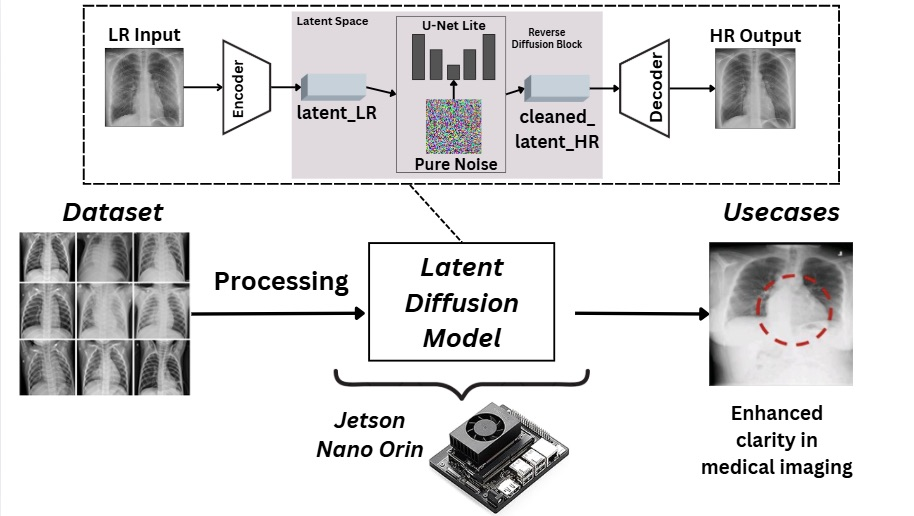
\includegraphics[width=1\textwidth]{Figs/modelmain.jpg}
\end{center}
\caption{The proposed model.}
\label{modelmain}
\end{figure}

\section{Individual Contributions and Responsibilities}

Overall, the project is progressing on schedule. Team communication is smooth and members are fulfilling their responsibilities on time.

\subsection{Collaboration}

The team uses a variety of different platforms for efficient communication and organization, as outlined in Table~\ref{platforms-table}. These collaboration strategies remain largely unchanged from those laid out in the Project Proposal.

Weekly meetings are held on Thursdays at 6:00 PM in the Bahen building on campus and Mondays at 9:00 PM over Google Meet. Meetings had originally been scheduled for Saturdays at 12 PM, but this proved to be an inconvenient time and was adjusted accordingly.

\begin{table}[h!]
\captionsetup{justification=centering}
\caption{Platforms used for team collaboration and project execution.}
\label{platforms-table}
\centering
\renewcommand{\arraystretch}{1.5}
\setlength{\tabcolsep}{6pt}
\begin{tabularx}{\textwidth}{
  @{} >{\raggedright\arraybackslash}p{2.2cm} 
  >{\raggedright\arraybackslash}p{3cm} 
  >{\raggedright\arraybackslash}X @{}
}
\toprule
\textbf{Platform} & \textbf{Purpose} & \textbf{Details of Use} \\
\midrule
Discord & Main communication & Daily updates; meeting scheduling; link sharing. \\[8pt]

Google Meet & Secondary communication & Virtual meetings. \\[8pt]

Google Drive & File hosting & Shared document editing; resource hub. \\[8pt]

GitHub & Code hosting & Version control; collaborative code editing. \\[8pt]

ClickUp & Project management & Shared Gantt chart; hub for deadlines; meeting schedules; task assignment. \\
\bottomrule
\end{tabularx}
\end{table}

\subsection{Task Management}

Each team member was assigned responsibility for two focus areas in the Project Proposal, as in Table~\ref{team-table}. A detailed breakdown of completed and future tasks is in Table~\ref{task-table}. Most tasks have been completed on time and some within a small margin of the due date. The team has not encountered any issues with teamwork or deadlines, and the project is on track to be completed in the time available.

The major remaining tasks are model performance improvement and edge deployment. Two team members are assigned to each task to provide redundancy in case of unexpected roadblocks.

\begin{table}[h]
\caption{Team member responsibilities and specialization areas.}
\label{team-table}
\begin{center}
\begin{tabular}{lll}
\toprule
\multicolumn{1}{c}{\bf Member} &
\multicolumn{1}{c}{\bf Primary Focus} &
\multicolumn{1}{c}{\bf Secondary Focus} \\
\midrule
A: Ayushi Agrawal   & Data Processing \& Evaluation     & Deployment testing, slide design \\
\addlinespace
B: Saaim Raad       & Model Architecture                & Dataset integration, training \& docs \\
\addlinespace
C: Md Nazmus Saad   & Diffusion \& Deployment           & Model training \& evaluation metrics \\
\addlinespace
D: Pakhi Gupta      & Documentation \& UI               & Data pairing, augmentation, visualization \\
\bottomrule
\end{tabular}
\end{center}
\end{table}

\begin{table}[h!]
\captionsetup{justification=centering}
\caption{Project task breakdown and responsible team members.}
\label{task-table}
\centering
\renewcommand{\arraystretch}{1.5} 
\setlength{\tabcolsep}{6pt}
\begin{tabularx}{\textwidth}{
  >{\centering\arraybackslash}p{1.2cm}   % Member narrower
  >{\raggedright\arraybackslash}X         % Tasks wide
  >{\centering\arraybackslash}p{1.8cm}   % Due narrower
  >{\centering\arraybackslash}p{1.8cm}   % Completed narrower
}
\toprule
\textbf{Member} & \textbf{Tasks} & \textbf{Due} & \textbf{Completed} \\
\midrule
A & Download data and extract to folder automatically; Create LR and HR pairs; Create PyTorch Dataset and Dataloaders using appropriate transformations & June 17 & June 20 \\[8pt]

D & Add data augmentation functionality to Dataset; Implement probabilistic random horizontal flip, rotations, resized crop and cutout consistently for LR and HR & June 22 & June 23 \\[8pt]

C & Build U-Net-Lite architecture; Implement diffusion scheduler & July 5 & July 7 \\[8pt]

B & Implement VAE encoder/decoder; Train initial model; Implement diffusion scheduler & July 9 & July 9 \\[12pt]

\multicolumn{4}{l}{\textbf{Upcoming Tasks}} \\
\addlinespace[8pt]

B, C & Additional hyperparameter tuning; Export model to ONNX & July 24 & \\[8pt]

C, B & Use TensorRT to quantize model and benchmark latency on Jetson & Aug 7 & \\[8pt]

A, C & Build an interface to show before/after on edge device & Aug 11 & \\[8pt]

D, A & Test model using evaluation metrics; Create final report and presentation & Aug 14 & \\
\bottomrule
\end{tabularx}
\end{table}


\section{Data Processing}

The dataset used is the publicly available NIH ChestX-ray14 dataset \citep{wang17} consisting of 112,120 1024x1024 images of chest X-rays from 30,805 unique patients.

The Indiana University Chest X-Ray Collection of more than 7000 images accessible through Open-i \citep{demner2016} will be used as new testing data. It contains both lateral and frontal view X-rays, as opposed to the NIH set which contains only frontal X-rays. This will ensure that the model can be tested on images completely different from its training data.

\subsection{Data Loading}

The following steps were used to obtain and process the dataset, of which a few sample images are shown in Figure~\ref{training_samples}:

\begin{enumerate}
    \item \textbf{Data downloading and organization:} A downloading script allows the user to download a specified number of batches from the dataset source, extracts them into the specified folder, and prevents overwriting of existing data.
    
    \item \textbf{Generating HR and LR image pairs:} The \texttt{generate\_downsampled\_pairs} function downsamples the original 1024x1024 images twice using OpenCV’s \texttt{resize} function with bicubic interpolation. The 256x256 downsampled image is saved into the \texttt{HR\_256} folder and the 64x64 version is saved into the \texttt{LR\_64} folder.
    
    \item \textbf{Creating a custom PyTorch dataset:} The \texttt{PairDataset} class reads images from their folders, transforms them into tensors of type \texttt{float32} and normalizes them to [-1,1] for faster training convergence. It assembles mini-batches of dimension B$\times$3$\times$64$\times$64 or B$\times$3$\times$256$\times$256 for input images and labels (ground truths) respectively.
    
    \item \textbf{Dataset splitting:} The \texttt{PairDataset} class also allows for configurable splits between train/validation/test data. A 70-20-10 split is currently in use, which provides 38,527 training, 10,907 validation, and 5,500 test images. One of the challenges here was to keep images from the same patient together, which was solved using careful parsing of filename while generating split indices.
\end{enumerate}

The same steps will be followed for testing on the new data (Indiana University). The only required change will be to set the data directory (a configurable argument) to the directory where the new data has been extracted, and to ensure images are cropped to squares before resizing.

\begin{figure}[h]
\begin{center}
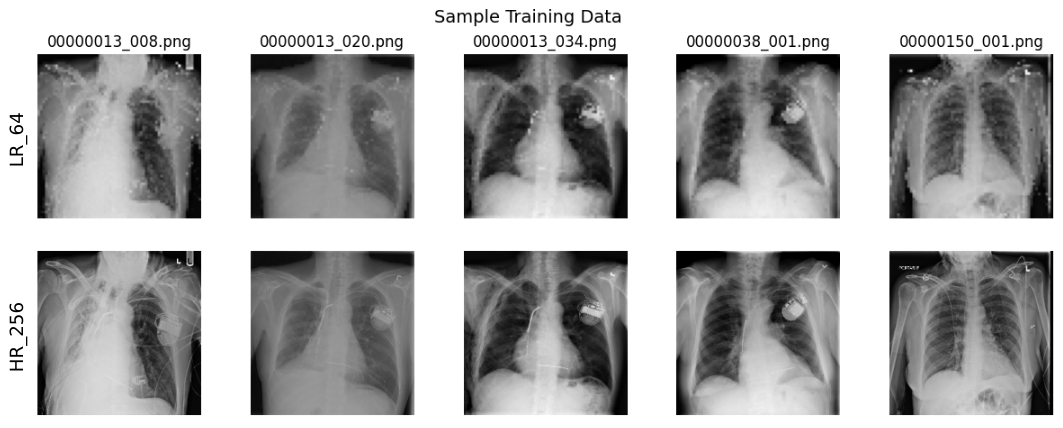
\includegraphics[width=1\textwidth]{Figs/training_samples.png}
\end{center}
\caption{Some random samples of the training data without data augmentation.}
\label{training_samples}
\end{figure}

\subsection{Data Augmentation}

To improve generalization and robustness, data augmentation was applied to 70\% of the training samples. This percentage was chosen based on empirical studies suggesting that moderate augmentation helps prevent overfitting while maintaining data fidelity, which is particularly important in the medical imaging domain where fine-grained details are critical \citep{athalye23, sanaat22}. Each augmentation was implemented considering spatial alignment, ensuring the LR and HR image pairs remained synchronized. The augmentation techniques used are as follows:

\begin{itemize}
    \item \textbf{Random Horizontal Flip (50\% chance):} Both the LR and HR images were flipped along the vertical axis using \texttt{torchvision.transforms.functional.hflip}. This augmentation helps the model become invariant to left-right orientation, which is useful for X-ray images where anatomical symmetry is common and directional bias can lead to misclassification.

    \item \textbf{Random Rotation (90\degree, 180\degree, or 270\degree):} Implemented using \texttt{F.rotate}, this augmentation rotates both images in discrete steps. These rotations simulate different acquisition angles, which can occur in real-world imaging scenarios due to variations in patient posture or X-ray machine positioning. Using discrete angles helps preserve anatomical integrity while still adding valuable diversity.

    \item \textbf{Random Resized Crop (80\% of original size):} A random crop of 80\% of the image was selected and then resized back to the original dimensions. The same crop coordinates were applied to both LR and HR images. This helps the model learn robust features across various subregions of the image, which is essential in X-rays where abnormalities can appear anywhere.

    \item \textbf{Cutout Augmentation (30\% chance):} A square patch (covering 20\% of the image size) was blacked out at a random location using direct tensor masking. This simulates occlusions or artifacts, such as medical markers or foreign objects, often present in X-rays. Training with cutout encourages the model to rely on surrounding context, improving resilience to incomplete data.
\end{itemize}

As shown in Figure~\ref{augmentations}, these augmentation techniques provide diverse and medically plausible variations during training.

While implementing these techniques, a few challenges were faced. Since the low- and high-resolution image pairs had different sizes, keeping them aligned during transformations like cropping meant the coordinates had to be scaled carefully. It was also important to avoid any unrealistic augmentations like color jitter and warping, which were left out to ensure the medical value of the X-rays was not compromised. Choosing to apply augmentation to around 70\% of the data helped strike a good balance between adding useful variation and still keeping enough original examples for the model to learn from accurately.

\begin{figure}[h!]
\centering
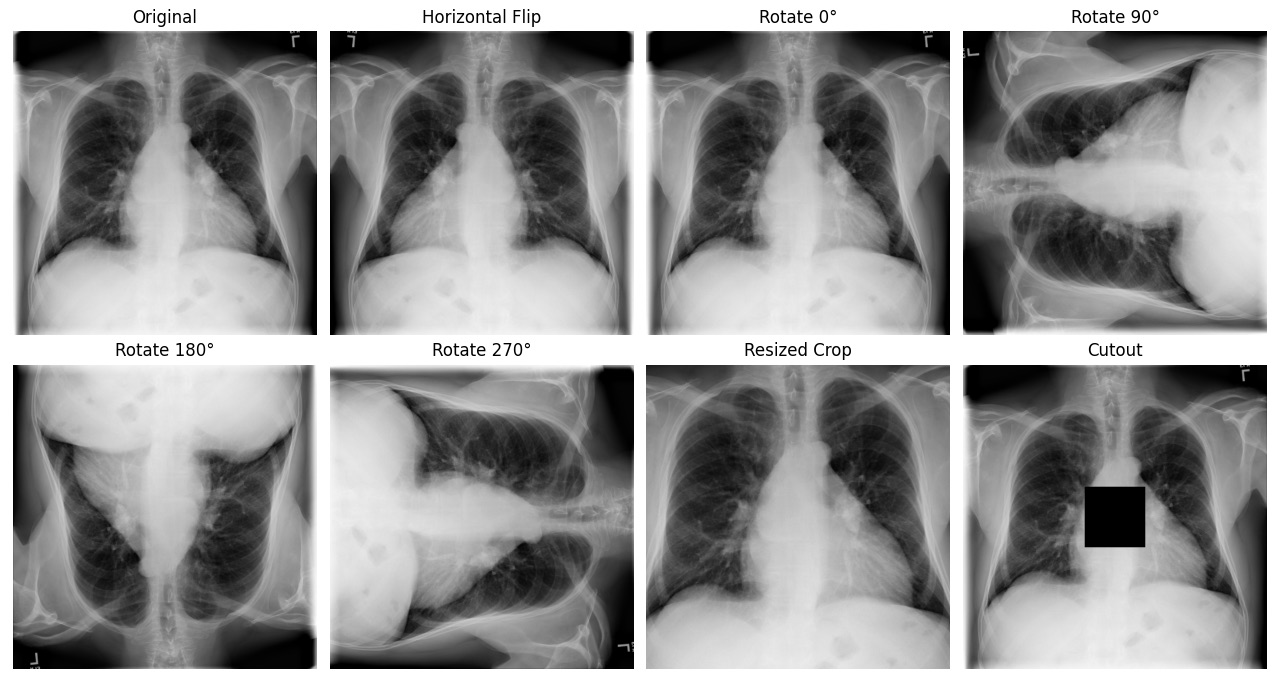
\includegraphics[width=0.9\textwidth]{Figs/augmentation.jpg}
\caption{Demonstration of augmentation techniques used in model training.}
\label{augmentations}
\end{figure}

\section{Baseline Model}

The baseline model that will be used to compare with our primary model is bicubic upsampling. First, the LR image was taken as input and resized to an HR image via bicubic upsampling. After that, PSNR, which quantifies the reconstruction quality based on pixel-wise errors and SSIM, which assesses perceptual quality by comparing luminance, contrast, and structural information, were computed (Figure~\ref{baseline}). The bicubic sampling is performed via PyTorch's \texttt{F.interpolate} function.

\begin{figure}[h]
\begin{center}
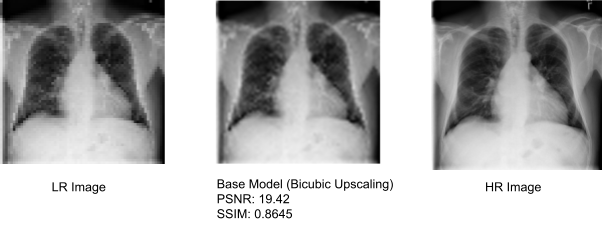
\includegraphics[width=1\textwidth]{progress/Figs/baseline.png}
\end{center}
\caption{One example showing the baseline models' improvements over the LR image and the computed PSNR/SSIM.}
\label{baseline}
\end{figure}


\section{Primary Model}

The primary model performs super-resolution on low-resolution chest X-rays using a latent diffusion-based architecture. As shown in Figure~\ref{model2}, the system includes a pretrained VAE, custom diffusion schedulers, and a custom U-Net, totaling 813,220 trainable parameters. All training was conducted on an NVIDIA GeForce RTX 4090.

\begin{figure}[h]
\begin{center}
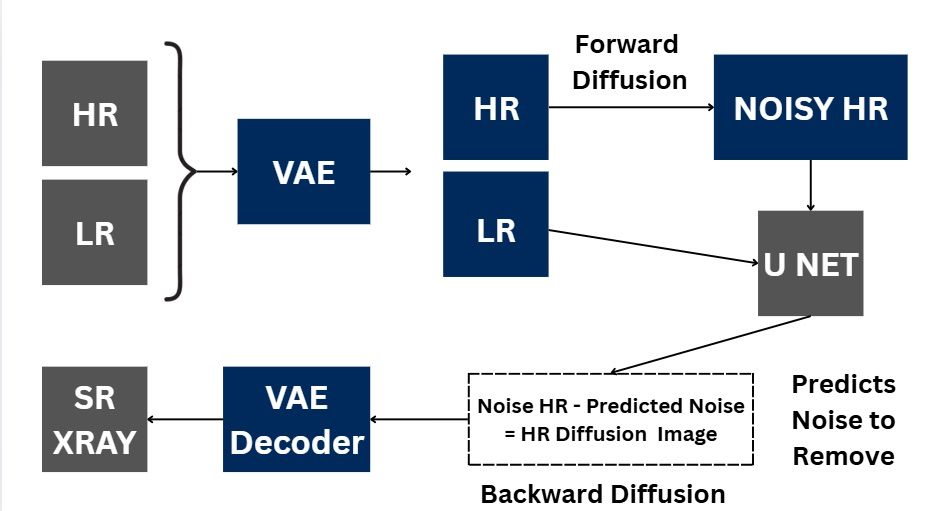
\includegraphics[width=1\textwidth]{progress/Figs/model2.jpg}
\end{center}
\caption{High level block diagram of architecture used for both training and inference.}
\label{model2}
\end{figure}

\subsection{Model Architecture and Design Choices}

\subsubsection{Latent Diffusion-Based Super-Resolution}

The model takes paired LR and HR images (3×64×64 and 3×256×256). LR images are first upsampled to 3×256×256 via bicubic interpolation, then both LR and HR images are encoded to latent space separately using Hugging Face’s pretrained AutoencoderKL VAE, yielding 4×32×32 latents by reducing spatial resolution 8× and expanding channels from 3 to 4.

\subsubsection{Forward Diffusion and Timestep Conditioning}

Training uses the forward diffusion process, where Gaussian noise is progressively added to the HR latent over multiple time steps. Rather than sequentially applying noise at each step, we use the closed-form DDPM formula for efficiency:
\[
z_t = \sqrt{\bar{\alpha}_t} \cdot z_0 + \sqrt{1 - \bar{\alpha}_t} \cdot \epsilon
\]
This closed form calculates the final noisy HR latent given some number of timesteps \( t \in [0, 300) \). The timestep \( t \) controls the noise level, as a higher \( t \) implies more steps that add noise. \( z_0 \) is the clean HR latent, \( \epsilon \sim \mathcal{N}(0, 1) \), and
\[
\bar{\alpha}_t = \prod_{i=1}^{t} (1 - \beta_i)
\]
with \( \beta \) linearly scheduled from 0.0001 to 0.02, as per the original DDPM paper \citep{ho20}. The noisy HR latent is concatenated with the LR latent to form an 8-channel tensor passed to the U-Net, alongside the timestep \( t \).

U-Net uses an encoder-decoder structure with skip connections (Figure~\ref{model3}) \citep{ronneberger2015unet}. Through conditioning available from the LR latent and \( t \), the U-Net learns to predict the noise added to the HR latent, trained using MSE loss against the true \( \epsilon \) added during the forward diffusion process.

\begin{figure}[h]
\begin{center}
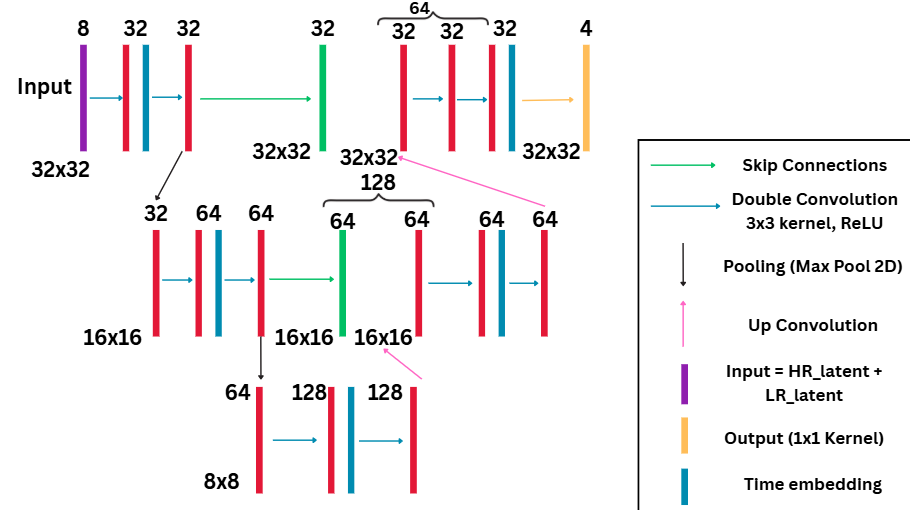
\includegraphics[width=1\textwidth]{progress/Figs/model3.png}
\end{center}
\caption{Structure of the U-Net.}
\label{model3}
\end{figure}

\subsubsection{Inference and Reverse Diffusion}

During inference, the process starts from pure Gaussian noise in latent space (\(4 \times 32 \times 32\)). Reverse diffusion is performed from \( t = 299 \) to \( 0 \), iteratively denoising with the trained U-Net. At each step, the LR latent is concatenated with the noisy HR latent, and the predicted \( \hat{\epsilon}_t \) is used to reverse the noise. After all steps, the final latent is decoded via the VAE to produce a \(3 \times 256 \times 256\) super-resolved image. PSNR is used to measure performance against ground-truth HR images, with bicubic interpolation as a baseline.

\subsection{Model Performance}

\subsubsection{Verifying Training Function}

To validate the implementation, the model was overfitted on a 10-image subset. After 500 epochs, the loss decreased to 0.144 but did not reach zero (Figure~\ref{overfitloss}), as diffusion models aim to predict stochastic noise rather than exact targets. The minimum MSE is lower-bounded by noise variance, VAE reconstruction error, and the KL-divergence term. Visually, the diffusion output surpassed bicubic upsampling (Figure~\ref{overfit}), confirming correct training behavior.

\begin{figure}[h]
\begin{center}
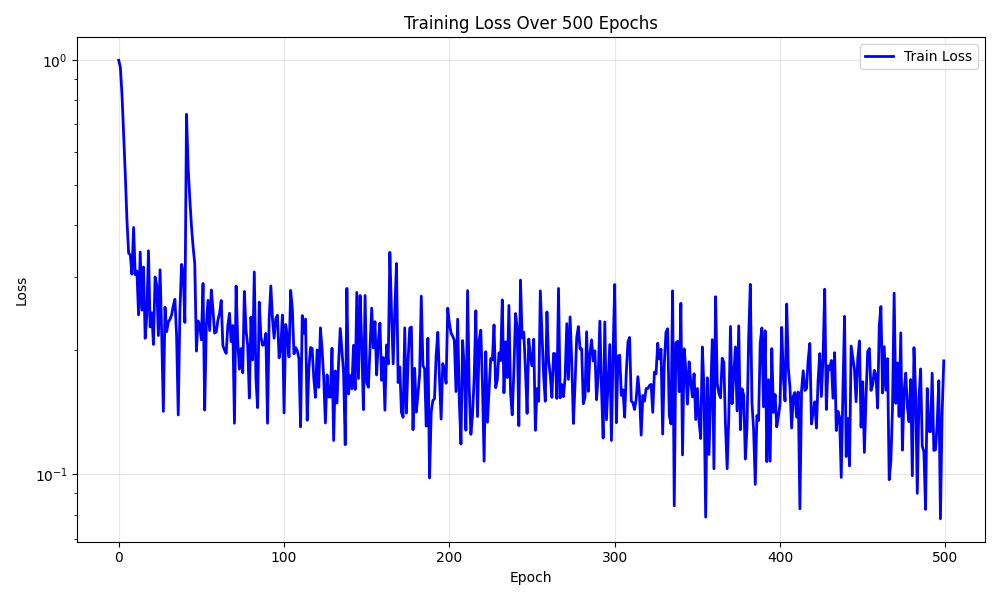
\includegraphics[width=1\textwidth]{progress/Figs/overfitloss.png}
\end{center}
\caption{Training loss graph during overfitting verification.}
\label{overfitloss}
\end{figure}

\begin{figure}[h]
\begin{center}
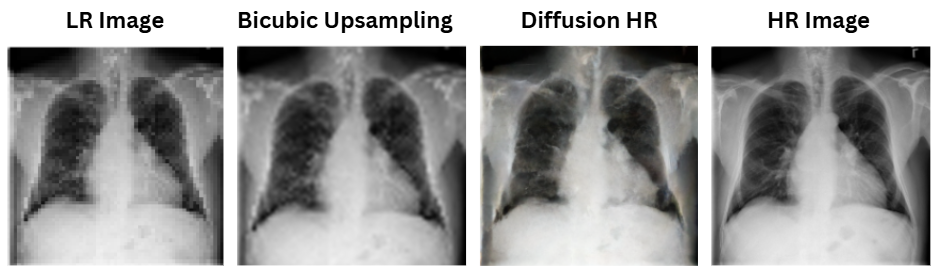
\includegraphics[width=1\textwidth]{progress/Figs/overfit.png}
\end{center}
\caption{Visual example of overfitting result, showing more clarity than the baseline.}
\label{overfit}
\end{figure}

\subsubsection{Model Version 1 Performance}

For this first full experiment, the dataset was split 70\% train, 20\% validation, and 10\% test. Training ran for 50 epochs, but only six of the twelve available data batches were loaded, so each epoch saw half the images (effective batch size = 9\,632). Both training and validation losses dropped quickly at the start and then flattened out near 0.187 by roughly epoch 20 (Figure~\ref{v1loss}).

\begin{figure}[h]
\begin{center}
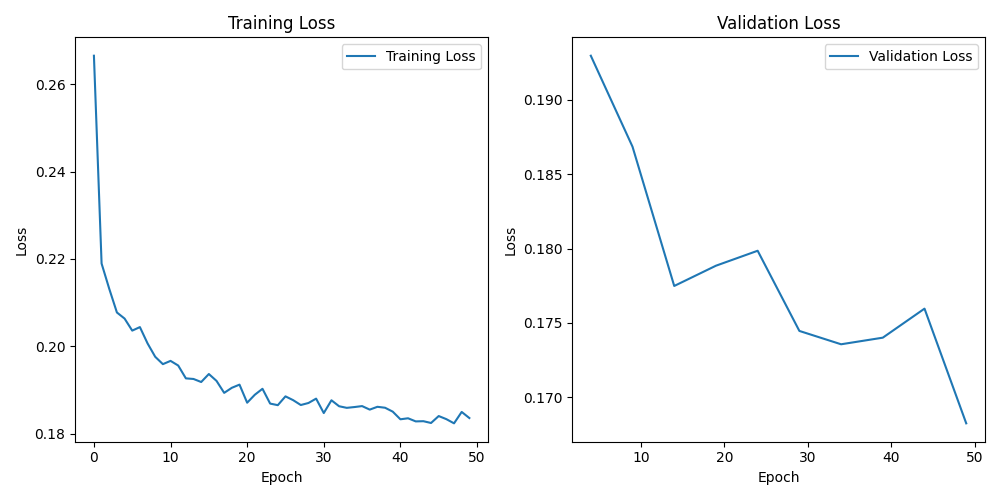
\includegraphics[width=1\textwidth]{progress/Figs/trainv1loss.png}
\end{center}
\caption{Training and validation curves for Version 1 of training.}
\label{v1loss}
\end{figure}

\begin{figure}[h]
\begin{center}
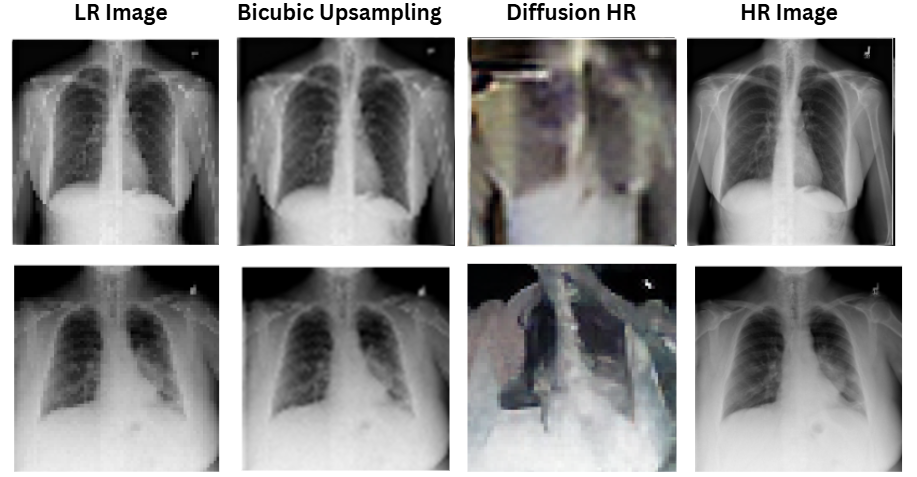
\includegraphics[width=1\textwidth]{progress/Figs/trainv1.png}
\end{center}
\caption{Visual example of training result.}
\label{v1}
\end{figure}

Although final outputs were blurrier than bicubic results, the model consistently generated lung-like structures from pure noise, indicating it had learned meaningful denoising patterns (Figure~\ref{v1}). Poor results were likely due to untuned hyperparameters, reduced data per epoch, a short training window, and limited U-Net capacity. Future experiments will include the full dataset, longer training, a deeper U-Net, and hyperparameter optimization (including $\beta$-scheduling) to improve output quality.

\subsection{Challenges}

Key challenges involved designing and integrating the diffusion scheduler with the VAE and U-Net. As a latent diffusion model, the system required a solid understanding of discrete-time stochastic processes and variational inference to generate images from pure noise. A significant portion of time was spent reading relevant literature and working through the underlying math to ensure correct implementation. As a result, only one full training run was completed (approximately 6 hours), leaving inadequate time for hyperparameter tuning. Although metrics such as PSNR, SSIM, and test loss are straightforward to compute for evaluating diffusion model outputs on the test set, they were not included due to time constraints but will be incorporated shortly for a more complete evaluation, and in order to better compare bicubic upsampling with latent diffusion.

\clearpage

\label{last_page}

\bibliography{APS360_ref}
\bibliographystyle{iclr2022_conference}

\end{document}
